% =====================================================================
% SECCIÓN 1: INTRODUCCIÓN, MOTIVACIÓN Y PROBLEMA
% =====================================================================

% ---------------------------------------------------------------------
% Diapositiva 1: Portada
% ---------------------------------------------------------------------
\begin{frame}[plain]
  \titlepage
  \note{
    Buenos días miembros del tribunal evaluador y docentes presentes. Hoy junto a Bruno Pace tenemos el agrado de presentar la defensa de nuestra tesina de grado para la Licenciatura en Ciencia de Datos de la Universidad del Gran Rosario, titulada: 'Detección temprana de indicios de depresión en publicaciones en español mediante procesamiento del lenguaje natural: Evaluación empírica de modelos contextuales y líneas base clásicas'.
  }
\end{frame}

% ---------------------------------------------------------------------
% Diapositiva 2: Contexto y Motivación
% ---------------------------------------------------------------------
\section{Comprensión del problema}

\begin{frame}{Contexto y motivación: salud pública y huella digital}
  
  \begin{columns}[T]
    \column{0.58\textwidth}
    \begin{itemize}
      \item \textbf{Crisis global de salud mental:} La depresión afecta a $\sim$5{,}2\,\% de los adultos del mundo (OMS, 2026) y es la principal causa de discapacidad persistente.
      \item \textbf{Brecha diagnóstica:} Hasta un 60\,\% de quienes padecen malestar afectivo no acceden a atención oportuna.
      \item \textbf{Huella digital en redes:} Señales lingüísticas y cambios conductuales en redes sociales meses antes de la primera consulta clínica.
      \item \textbf{Asimetría del español:} La investigación en PLN se concentra en \textbf{inglés}; en español los corpus anotados son escasos y de acceso restringido.
    \end{itemize}

    \column{0.40\textwidth}
    \begin{center}
      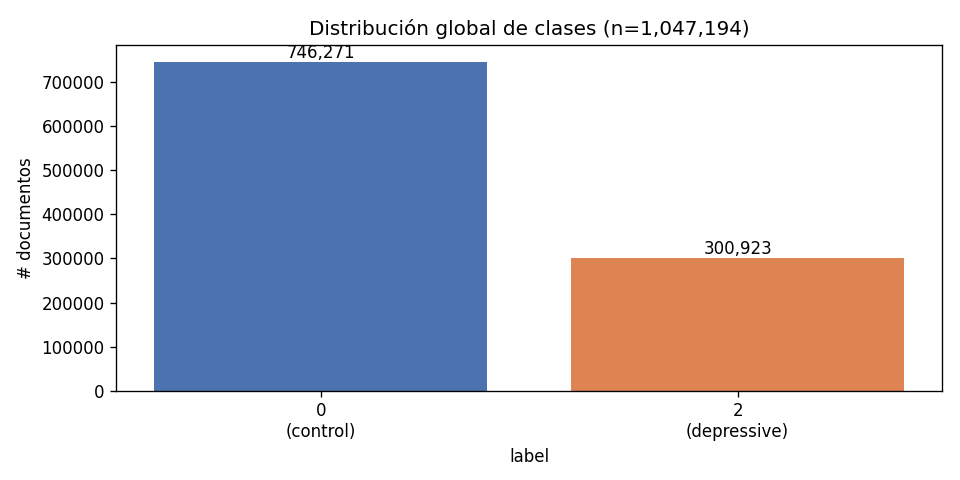
\includegraphics[width=\textwidth,height=0.34\textheight,keepaspectratio]{eda_02_distribucion_clases.png}
      \vskip-0.05cm
      {\tiny\color{ugrGris}Figura 1: Distribución global de clases en el corpus (1{,}31M de textos).\par}
    \end{center}
  \end{columns}

  \vskip0.05cm
  \ugrblock{Delimitación ética y alcance computacional}{
    Desarrollamos clasificadores estadísticos de texto como apoyo al cribado poblacional. El sistema \textbf{no} constituye ni sustituye un diagnóstico clínico.
  }

  \note{
    La depresión es una crisis de salud pública de escala mundial. Las redes sociales representan un canal donde los usuarios manifiestan cambios conductuales y léxicos tempranos. Sin embargo, existe una notable asimetría: casi toda la investigación en PLN se realiza en inglés, mientras que en español los recursos abiertos son mínimos. Aclaramos desde el inicio que el trabajo se enmarca en la clasificación supervisada para cribado preventivo, no en el diagnóstico médico.
  }
\end{frame}

% ---------------------------------------------------------------------
% Diapositiva 3: Planteamiento del Problema
% ---------------------------------------------------------------------
\begin{frame}{Planteamiento del problema y preguntas de investigación}
  \framesubtitle{Pregunta central y dimensiones metodológicas en Ciencia de Datos}

  \ugrblock{Pregunta central de investigación}{
    \textit{¿Es posible desarrollar un clasificador supervisado en Ciencia de Datos que, a partir de texto en español a nivel de publicación, distinga publicaciones con indicios de depresión frente a controles con un desempeño predictivo significativamente superior al de las representaciones clásicas, manteniendo robustez y evaluación no sesgada?}
  }

  \vskip0.05cm
  \begin{columns}[T]
    \column{0.49\textwidth}
    \ugrblock{1. Transferencia translingüística}{
      ¿Permite la traducción automática neuronal (EN$\to$ES) aumentar los datos de entrenamiento y beneficiar la detección en el dominio nativo en español?
    }
    \column{0.49\textwidth}
    \ugrblock{2. Evaluación por unidad de análisis}{
      ¿Cómo cambia el rendimiento predictivo al evaluar publicaciones individuales frente a perfiles completos de usuario?
    }
  \end{columns}

  \vskip0.05cm
  \begin{itemize}
    \item \textbf{Unidad de análisis:} Establecer una distinción metódica formal entre la predicción a \textbf{nivel de publicación} (tweet individual) y a \textbf{nivel de usuario} (perfil histórico acumulado).
  \end{itemize}

  \note{
    Formulamos una pregunta central con rigor epistemológico: contrastar si las arquitecturas Transformer contextuales superan efectivamente a los modelos clásicos en español bajo un marco no sesgado. A partir de allí exploramos si la traducción automática transfiere mejoras al dominio nativo.
  }
\end{frame}
